\documentclass{article}
\usepackage[utf8]{inputenc}
\usepackage{graphicx}
\graphicspath{ {images/} }
\usepackage[english]{babel}
\usepackage[utf8]{inputenc}
\usepackage{amsmath}
\usepackage{graphicx}
\usepackage{listings}
\usepackage{enumerate}
\usepackage{float}



\begin{titlepage}
\begin{document}



\ \\ \ \\ \ \\ \ \\ \ \\ %

\begin{center}
\huge{Laboratorio }\\
\huge{de}\\
\huge{Redes}\\
\end{center}

\ \\ \ \\ \ \\ \ \\ \ \\ \ \\ \ \\ \ \\ \ \\ \ \\%

\begin{center}
\large{{Integrantes}} \\
\large{Eva Moya 201173597-8} \\
\large{Sebasti\'an Tapia  201173599-4}\\
\large{ eva.moya@alumnos.usm.cl }\\
\large{sebastian.tapia@alumnos.usm.cl}\\
\end{center}
\end{titlepage}


\section{Respuestas de la herramienta}

Al introducir las direcciones en la aplicación "Open Visual Traceroute", se obtuvieron diferentes repuestas para cada una de ellas, en otras palabras, los paquetes enviados tomaron diferentes "rutas", sin embargo, algunos puntos de estas rutas se repiten.\\
A continuación se muestran las imágenes en donde se puede apreciar las rutas tomadas en cada uno de los casos, estas rutas se representan como una lista al lado derecho de la fotografía.\\

\begin{figure}[H]
\centering
\includegraphics[width=1\textwidth]{moodle_inf_cl.png}
\end{figure}


\begin{figure}[H]
\centering
\includegraphics[width=1\textwidth]{google_cl.png}
\end{figure}


\begin{figure}[H]
\centering
\includegraphics[width=1\textwidth]{cime_cl.png}
\end{figure}


\begin{figure}[H]
\centering
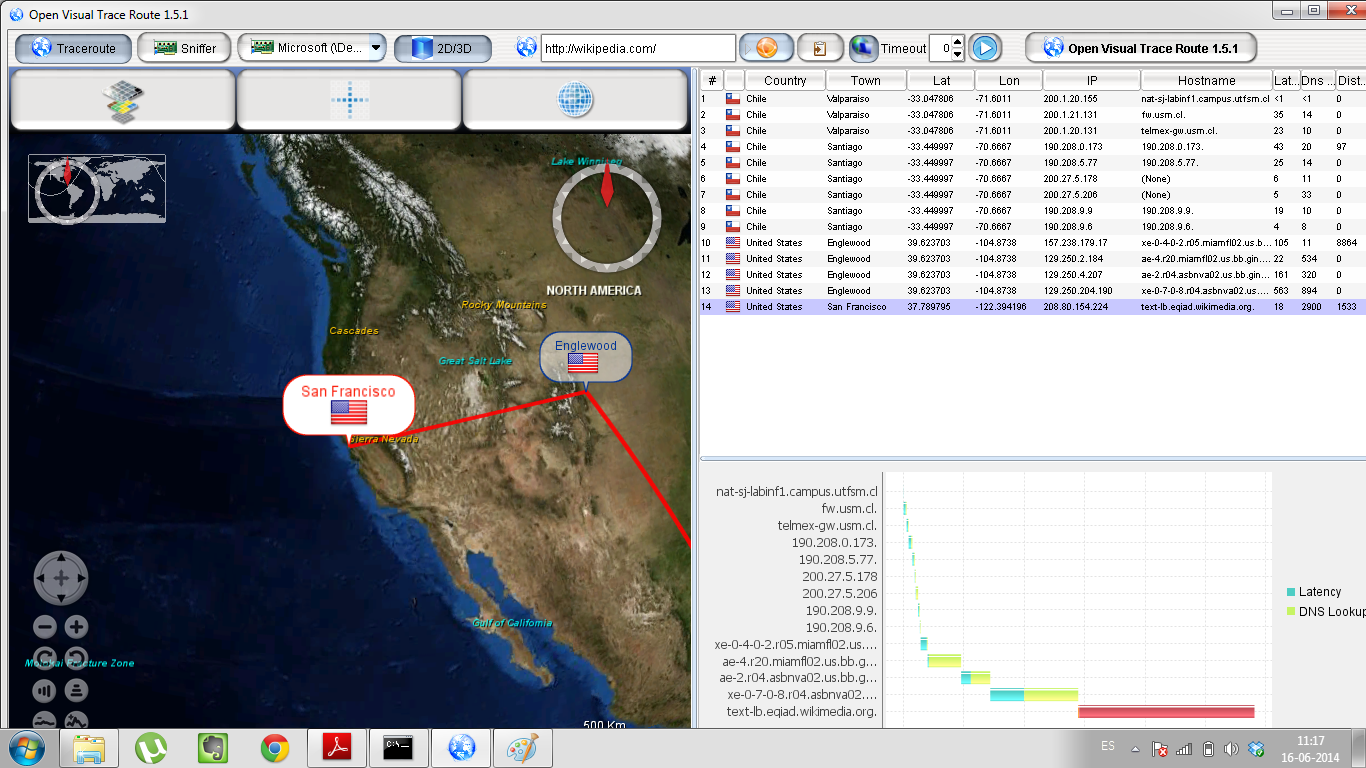
\includegraphics[width=1\textwidth]{wikipedia.png}
\end{figure}



\begin{figure}[H]
\centering
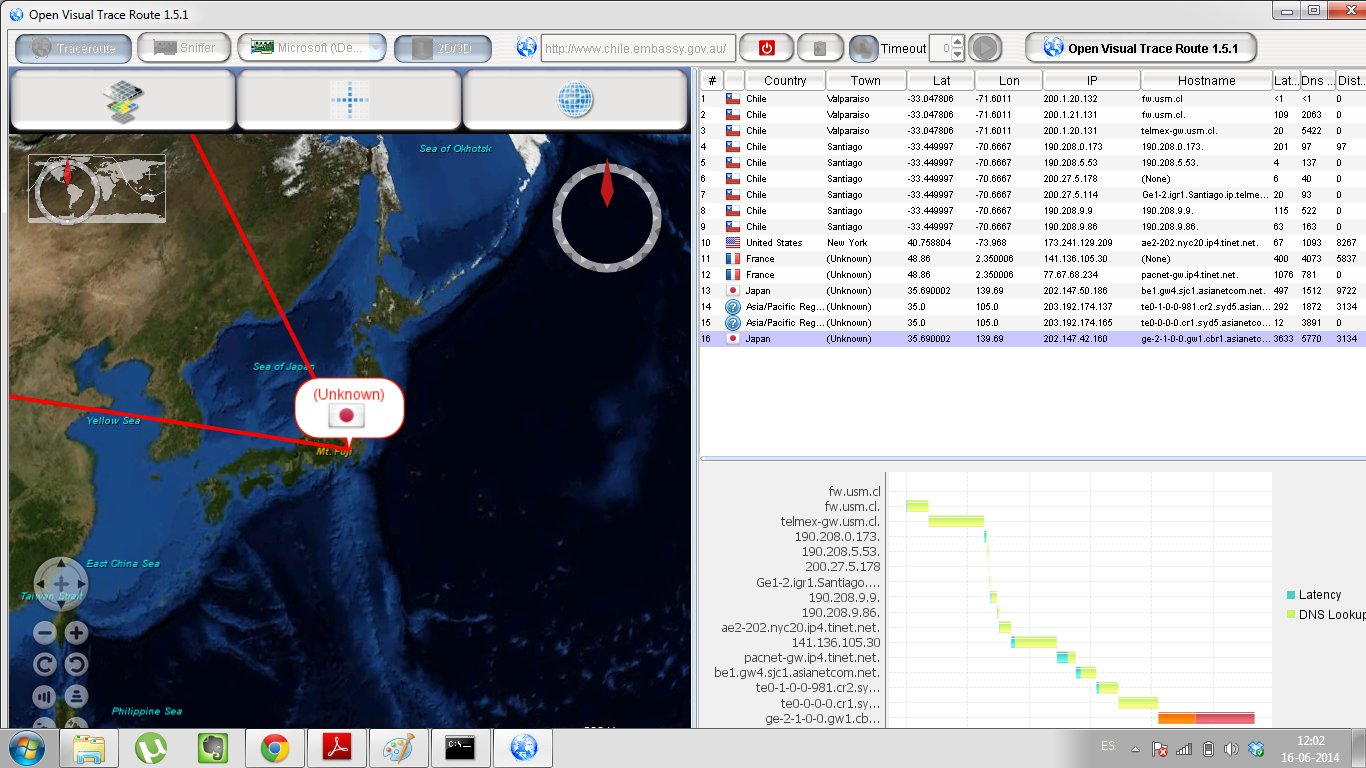
\includegraphics[width=1\textwidth]{embajada.png}
\end{figure}




\section{¿Por qué los paquetes toman las rutas que aparecen en la herramienta?}

Se puede apreciar en las imágenes anteriores, que los paquetes enviados por cada una de las direcciones toman diferentes rutas y esto se debe básicamente a que internet es una "red de redes" en donde los paquetes viajan por cada router y por cada ISP hasta llegar a su destino según la "mejor" ruta determinada para ellos (ruta obtenida a través de un protocolo de enrutamiento).\\

Los protocolos de enrutamiento difieren según el viaje de cada paquete, en el caso de que estos paquetes viajen entre routers de un mismo AS de un ISP, el protocolo más comunmente utilizado es de tipo "Link-State" llamado "OSPF", el cual se encarga de encontrar la primera ruta más corta. Por otro lado, en el caso de que los paquetes viajen entre distintos AS, el protocolo de ruteo utilizado es el llamado "BGP" el cual se encarga de encontrar una ruta adecuada según ciertas reglas y políticas de la red.\\


También se puede apreciar en las imágenes que algunos de los puntos geográficos se repiten en las rutas obtenidas por las distintas direcciones y esto se debe a los enlaces nacionales e internacionales fijos y específicos que tiene Chile para conectarse a internet, los cuales se conectan a otros enlaces y así logran viajar de continente a continente.\\


\section{¿Como viajan los paquetes de un continente a otro?}

Los paquetes viajan de un continente a otro por medio de enlaces o conexiones internacionales que corresponden a diversas redes de cables submarinos de Fibra Óptica, en donde un 90\% aproximadamente del tráfico de Internet circula a tráves de estos cables.\\

A pesar de que los cables de fibra optica tienen una gran tolerancia a las interferencias y a la pérdida de señal, es casi imposible evitar que se debilite la señal de transmisión o que se pierda al viajar por tan largas distancias. Para evitar este tipo de problemas la red cuenta con "Repetidores" conectados cada cierta distancia a los cables de fibra óptica, estos repetidores son unos dispositivos electrónicos los cuales se encargan de retransmitir a una potencia más alta una señal debil o de bajo nivel.\\


Actualmente Chile está conectado con el resto del mundo por medio de los siguientes cables activos: \\

Cable Panamericano (PanAm), al que se conecta en Arica, funciona a una velocidad de 70 Gbps. y abarca 7.050 km.\\

Cable South American Crossing (SAC)/Latin American Nautilus (LAN), que tiene conexión desde Valparaíso a una velocidad de 3.84 Tbps. y abarca 20.000 km. \\

Cable South America-1 (SAm-1), que tiene conexión desde Arica y Valparaíso, funciona a 1.92 Tbps. y abarca 25.000 km.\\

A continuación de muestra una imagen con todos los cables submarinos de fibra óptica:

\begin{figure}[H]
\centering
\includegraphics[width=1\textwidth]{red_de_redes.png}
\end{figure}

\section{¿Qué es específicamente la Fibra Óptica?}

La fibra óptica es un medio de transmisión de datos, se trata mas bien de un hilo muy fino de material transparente (como vidrio o materiales plásticos), en el cual se envían pulsos de luz que representan los datos a transmitir, la fuente de luz puede ser un láser o un LED.

Los cables de fibras ópticas son empleados habitualmente en redes de datos, más apliamente en las telecomunicaciones, ya que gracias a su inmunidad a las interferencias electromagnéticas y a su flexibilidad, permiten enviar una gran cantidad de datos en una mayor distancia y a gran velocidad.\\


\section{¿Cómo se conectaron los continentes en el principio de los tiempos?}

Los continentes en "el principio de los tiempos" se conectaron igual que en la actualidad, a través de cables submarinos.

Todo comenzó en 1850 con la expansión del telégrafo, ya que surgió la necesidad de conectar dos países separados por mar, Francia e Inglaterra. Para suplir esta necesidad se tendió un cable de cobre submarino entre los dos países, este cable no fué de mucha ayuda ya que las señales sufrían retardos, esto sumado a los rebotes y ausencia de blindaje del cobre, la señal se hacía irreconocible. Este cable duró más o menos un año, ya que se rompió debido a que un pescador enganchó sus redes en él.

Luego de la avería de este primer cable, los ingenieros de la época debían enlazar otra vez Francia e Inglaterra, pero esta vez recubrieron los cables con "Gutapercha" logrando que los cables funcionaran bien bajo el agua. Con este "gran decubrimiento" se empezó a expandir aún más la red de telégrafos, logrando enlazar continentes, primero fue Europa y África, luego de unos años se logró enlazar América y Europa, cruzando el Océano Atlántico.\\

EL "cable trasatlántico" se averió poco despúes de su implementación y luego de 6 años lograron levantar el servicio con un nuevo cable con blindaje mas robusto y resistente, luego de esto serían 15 los cables que cruzarían los Atlántico para unir América con Europa.\\

En la década de los 60 aparece el "cable Coaxial", el cual es utilizado como base para la construcción de comunicaciones internacionales, los cuales son utilizados hasta la década de los 80 aproximadamente.\\

A mediados de los 80 y hasta el día de hoy, se comienza a desplegar la  contrucción de redes con cables de "Fibra Óptica".






\end{document}



